\documentclass[border=3pt]{standalone}
% Preâmbulo compartilhado pelos diagramas TikZ da aula 7 de IHR (Emoção)
\usepackage[T1]{fontenc}
\usepackage[utf8]{inputenc}
\usepackage{lmodern}
\usepackage{amsmath}
\usepackage{xcolor}
\usepackage{tikz}
\usetikzlibrary{arrows.meta,angles,quotes,decorations.pathmorphing,decorations.pathreplacing,calc,
                positioning,shapes.geometric,shapes.misc,backgrounds,fit,
                math}

% Paleta (mesma dos SVGs originais)
% Paleta da disciplina de IHR: acento azul (#1A6FB5), cor de destaque do tema.
% (o nome "dblue" é mantido para não alterar todos os diagramas)
\definecolor{dblue}{HTML}{1A6FB5}
\definecolor{dorange}{HTML}{B3541E}
\definecolor{dgreen}{HTML}{4A7C59}
\definecolor{dred}{HTML}{9C4B4B}
\definecolor{dcream}{HTML}{F4F1EA}
\definecolor{dshade}{HTML}{DDD7C9}

% Função gaussiana (não normalizada por padrão de escala visual)
\pgfmathdeclarefunction{gauss}{3}{%
  \pgfmathparse{1/(#3*sqrt(2*pi))*exp(-((#1-#2)^2)/(2*#3^2))}%
}

% Estilos comuns (prefixo d... para não colidir com chaves internas do pgf)
\tikzset{
  >={Stealth[length=2mm]},
  dguide/.style={gray!55, dashed, line width=0.4pt},
  daxis/.style={gray!60, line width=0.7pt, ->},
  dbody/.style={fill=black!3, draw=black!80, line width=1pt},
  dacc/.style={draw=dblue, line width=1pt},
  dlbl/.style={black!55, font=\small},
  dsub/.style={black!45, font=\footnotesize},
  dstate/.style={circle, draw=black!80, fill=dcream, line width=1pt,
                 minimum size=17mm, font=\large, inner sep=1pt},
  dobs/.style={circle, draw=black!80, fill=dshade, line width=1pt,
               minimum size=14mm, font=\large, inner sep=1pt},
  dbox/.style={rounded corners=2pt, draw=black!80, fill=dcream, line width=1pt,
               align=center, inner sep=6pt},
  dop/.style={circle, draw=black!80, fill=white, line width=1pt,
              minimum size=6mm, inner sep=0pt, font=\small},
  dtrans/.style={->, dblue, line width=1pt},
  dmeas/.style={->, dorange, line width=1pt},
  dcurve/.style={line width=1pt, dblue},
  dcurveb/.style={line width=1.4pt, dorange},
}

\begin{document}
\hyphenpenalty=10000 \exhyphenpenalty=10000 \tolerance=9999 \emergencystretch=3em
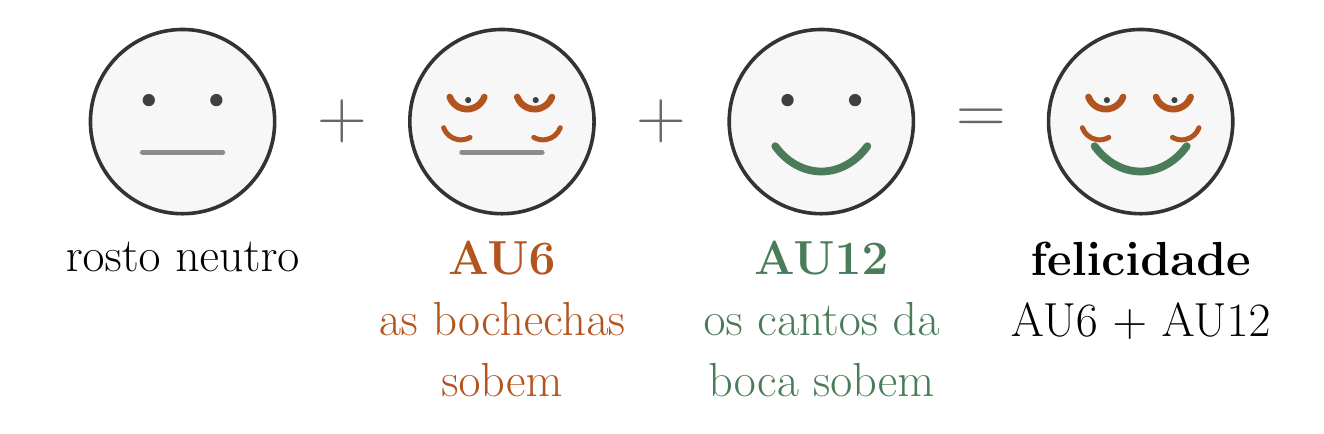
\begin{tikzpicture}[x=0.78cm,y=0.78cm]

  \tikzset{lab/.style={font=\LARGE, align=center, text width=3.7cm, anchor=north},
           op/.style={font=\Huge\bfseries, black!60}}
  \newcommand{\base}[1]{\draw[dbody, line width=1.3pt] (#1,0) circle (1.5);}
  \newcommand{\eyes}[1]{\fill[black!75] (#1-0.55,0.35) circle (0.1) (#1+0.55,0.35) circle (0.1);}
  \newcommand{\neutralmouth}[2]{\draw[#2, line width=2pt, line cap=round] (#1-0.65,-0.5) -- (#1+0.65,-0.5);}
  \newcommand{\cheeks}[1]{% AU6: olhos apertados e bochechas sobem
      \draw[dorange, line width=2.4pt, line cap=round] (#1-0.85,0.4) arc (200:340:0.3) (#1+0.25,0.4) arc (200:340:0.3);
      \draw[dorange, line width=1.8pt, line cap=round] (#1-0.95,-0.1) arc (200:300:0.3) (#1+0.95,-0.1) arc (340:240:0.3);}
  \newcommand{\sorriso}[1]{\draw[dgreen, line width=2.8pt, line cap=round] (#1-0.75,-0.4) .. controls (#1-0.35,-0.95) and (#1+0.35,-0.95) .. (#1+0.75,-0.4);}

  % 1. neutro
  \base{0} \eyes{0} \neutralmouth{0}{black!45}
  \node[lab] at (0,-1.8) {rosto neutro};
  \node[op] at (2.6,0) {$+$};

  % 2. AU6
  \base{5.2} \fill[black!75] (5.2-0.55,0.35) circle (0.05) (5.2+0.55,0.35) circle (0.05) ; \cheeks{5.2} \neutralmouth{5.2}{black!45}
  \node[lab, dorange] at (5.2,-1.8) {\textbf{AU6}\\ as bochechas sobem};
  \node[op] at (7.8,0) {$+$};

  % 3. AU12
  \base{10.4} \eyes{10.4} \sorriso{10.4}
  \node[lab, dgreen] at (10.4,-1.8) {\textbf{AU12}\\ os cantos da boca sobem};
  \node[op] at (13.0,0) {$=$};

  % 4. felicidade
  \base{15.6} \fill[black!75] (15.6-0.55,0.35) circle (0.05) (15.6+0.55,0.35) circle (0.05); \cheeks{15.6} \sorriso{15.6}
  \node[lab, black] at (15.6,-1.8) {\textbf{felicidade}\\ AU6 + AU12};

\end{tikzpicture}
\end{document}
